%!TEX TS-program = xelatex
\documentclass[12pt]{article}
\usepackage[utf8]{inputenc}

% \usepackage[english, russian]{babel} % выбор языка для документа
% \usepackage[utf8]{inputenc} % задание utf8 кодировки исходного tex файла
% \usepackage[X2,T2A]{fontenc}        % кодировка

\usepackage{fontspec}         % пакет для подгрузки шрифтов
\setmainfont{Arial}       % задаёт основной шрифт документа



\usepackage{verbatim}
\usepackage{lastpage}
\usepackage{epsfig}
\usepackage{graphicx}
\usepackage{float}
\usepackage{subfigure}
%\usepackage{overcite}
\usepackage{psfrag}
\usepackage{ifthen}
\usepackage{amsmath}
\usepackage{xcolor}
\usepackage{hyperref}
%\usepackage{cleveref}

\usepackage{indentfirst}

\textwidth=6.5in
\textheight=9in
\topmargin=-0.25in
\headheight=0in
\headsep=0in
\topskip=0in
\oddsidemargin=0in
\evensidemargin=0in

\newcommand{\PHNote}[1]{\ColorNote{red}{PH}{#1}}


 \usepackage{multirow}

\usepackage[backend=biber, style=numeric-comp,
	sorting=ynt,  
	defernumbers=true,
	 babel=other]{biblatex}

\addbibresource{references.bib}


\usepackage{enumitem}
\setenumerate[1]{label={(\alph*)}} 



\usepackage{amsmath,amsfonts,amssymb,amsthm,mathtools} % AMS
\usepackage{icomma} 
\mathtoolsset{showonlyrefs=true} % Показывать номера только у тех формул, на которые есть \eqref{} в тексте.
%\usepackage{euscript}	 % Шрифт Евклид
%\usepackage{mathrsfs} % Красивый матшрифт
\usepackage{enumitem}
\usepackage{siunitx}
\usepackage{tikz} % To generate the plot from csv
\usepackage{pgfplots}

\usepackage{hyperref}

%%% Заголовок

\newcommand{\latinword}[1]{\textsf{\itshape #1}}%


\usepackage{indentfirst}
\usepackage{fancyvrb}

\usepackage{mathtools}


%\usepackage[noae]{Sweave}

\tolerance=10000
\emergencystretch=\maxdimen
\widowpenalty=10000
\clubpenalty=10000 
%\hyphenpenalty=10000
%\hbadness=10000

\usepackage{graphicx}
\usepackage{float} 
 

\usepackage{pgfplots}
\pgfplotsset{compat=newest}

\usepackage{tikz}
\usetikzlibrary{calc}
\usetikzlibrary{quotes,angles}
\usetikzlibrary{arrows}
\usetikzlibrary{arrows.meta}
\usetikzlibrary{positioning,intersections,decorations.markings}

\usepackage{tkz-euclide} 


\newcommand{\grid}{\draw[color=gray,step=1.0,dotted] (-2.1,-2.1) grid (7.6,6.1)}

\newcommand{\ba}{\boldsymbol{a}}
\newcommand{\bb}{\boldsymbol{b}}
\newcommand{\bc}{\boldsymbol{c}}
\newcommand{\bd}{\boldsymbol{d}}
\newcommand{\bx}{\boldsymbol{x}}
\newcommand{\bv}{\boldsymbol{v}}


%\tikzset{>=latex}





\colorlet{veca}{red}
\colorlet{vecb}{blue}
\colorlet{vecc}{olive}


\usepackage[outline]{contour}

\usetikzlibrary{patterns}

\begin{document}


\section{Лекция 1}

\subsection{R1.1}


\begin{tikzpicture}[
scale=1,
MyPoints/.style={draw=blue,fill=white,thick},
Segments/.style={draw=blue!50!red!70,thick},
MyCircles/.style={green!50!blue!50,thin}, 
every node/.style={scale=1}
]
\grid;
\clip (-2.5,-2.5) rectangle (7.5,5.5);


%\draw[->, >=stealth] (-1,0)--(6.5,0) node[right]{$x_1$};
\draw[-{Latex[length=4.5mm, width=2.5mm]}, >=stealth] (0,-1)--(0,5) node[above left]{$x_2$};

\draw[-{Latex[length=4.5mm, width=2.5mm]}, >=stealth] (-1,0)--(6.5,0) 
node[right]{$x_1$};


%{\verb!->!new, arrowhead = 2mm, line width=4pt}
%, arrowhead = 3mm
%, arrowhead = 0.2

% Feel free to change here coordinates of points A and B
\pgfmathparse{0}		\let\Xa\pgfmathresult
\pgfmathparse{0}		\let\Ya\pgfmathresult
\coordinate (A) at (\Xa,\Ya);

\pgfmathparse{4}		\let\Xb\pgfmathresult
\pgfmathparse{3}		\let\Yb\pgfmathresult
\coordinate (B) at (\Xb,\Yb);

\pgfmathparse{4}		\let\Xc\pgfmathresult
\pgfmathparse{0}		\let\Yc\pgfmathresult
\coordinate (C) at (\Xc,\Yc);


% Let I be the midpoint of [AB]
\pgfmathparse{(\Xb+\Xa)/2} \let\XI\pgfmathresult
\pgfmathparse{(\Yb+\Ya)/2} \let\YI\pgfmathresult
\coordinate (I) at (\XI,\YI);	


\draw[-{Latex[length=4.5mm, width=2.5mm]}, >=stealth, vecb,thick] (A)--(B) node[midway,above]{$\bx$};

\draw[black, dashed, thick] (B)--(C) node[midway,right]{$3$};

\draw[black] (A)--(C) node[midway,below]{$4$};

\tkzMarkRightAngle[size=.3](A,C,B) 

\node [above right,darkgray] at (1,3.5) {$\bx=\left(\begin{array}{l}4 \\ 3\end{array}\right) \quad \|\bx\|=\sqrt{3^{2}+4^{2}}=5 $};

\end{tikzpicture}



\subsection{R1.2}



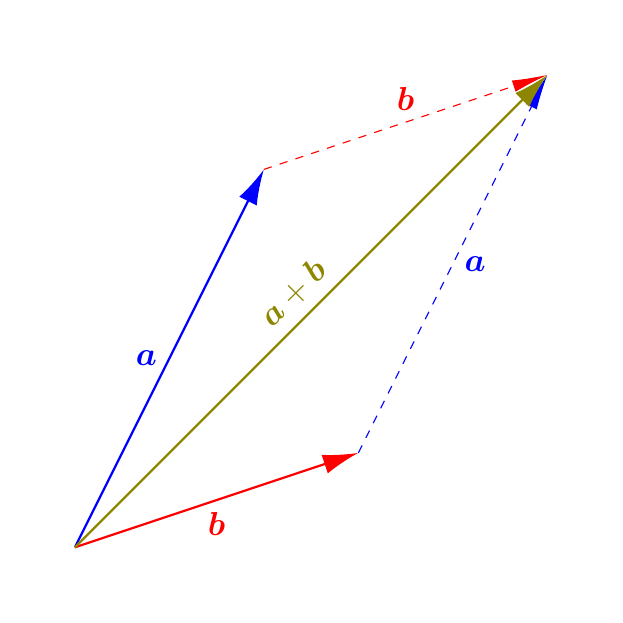
\begin{tikzpicture}[
scale=1.2,
MyPoints/.style={draw=blue,fill=white,thick},
Segments/.style={draw=blue!50!red!70,thick},
MyCircles/.style={green!50!blue!50,thin}, 
every node/.style={scale=1.2}
]
%\grid;
\clip (-.5,-.5) rectangle (5.5,5.5);


%%\draw[->, >=stealth] (-1,0)--(6.5,0) node[right]{$x_1$};
%\draw[-{Latex[length=4.5mm, width=2.5mm]}, >=stealth] (0,-1)--(0,5) node[above left]{$x_2$};
%
%\draw[-{Latex[length=4.5mm, width=2.5mm]}, >=stealth] (-1,0)--(6.5,0) 
%node[right]{$x_1$};

% Feel free to change here coordinates of points A and B
\pgfmathparse{0}		\let\Xa\pgfmathresult
\pgfmathparse{0}		\let\Ya\pgfmathresult
\coordinate (A) at (\Xa,\Ya);

\pgfmathparse{2}		\let\Xb\pgfmathresult
\pgfmathparse{4}		\let\Yb\pgfmathresult
\coordinate (B) at (\Xb,\Yb);

\pgfmathparse{3}		\let\Xc\pgfmathresult
\pgfmathparse{1}		\let\Yc\pgfmathresult
\coordinate (C) at (\Xc,\Yc);

\pgfmathparse{5}		\let\Xd\pgfmathresult
\pgfmathparse{5}		\let\Yd\pgfmathresult
\coordinate (D) at (\Xd,\Yd);



% Let I be the midpoint of [AB]
\pgfmathparse{(\Xb+\Xa)/2} \let\XI\pgfmathresult
\pgfmathparse{(\Yb+\Ya)/2} \let\YI\pgfmathresult
\coordinate (I) at (\XI,\YI);	


\draw[-{Latex[length=4.5mm, width=2.5mm]}, >=stealth, vecb,thick] (A)--(B) node[midway,left]{$\ba$};

\draw[-{Latex[length=4.5mm, width=1.5mm]}, >=stealth, vecb,dashed] (C)--(D) node[midway,right]{$\ba$};


\draw[-{Latex[length=4.5mm, width=2.5mm]}, >=stealth, veca,thick] (A)--(C) node[midway,below]{$\bb$};

\draw[-{Latex[length=4.5mm, width=1.5mm]}, >=stealth, veca,dashed] (B)--(D) node[midway,above]{$\bb$};


\draw[-{Latex[length=4.5mm, width=2.5mm]}, >=stealth, vecc,thick] (A)--(D) node[midway,above, sloped]{$\ba+\bb$};


\end{tikzpicture}


\subsection{R1.3}



\begin{tikzpicture}[
scale=1.2,
MyPoints/.style={draw=blue,fill=white,thick},
Segments/.style={draw=blue!50!red!70,thick},
MyCircles/.style={green!50!blue!50,thin}, 
every node/.style={scale=1.2}
]
%\grid;
\clip (-.5,-.5) rectangle (5.5,5.5);

\pgfmathparse{0}		\let\Xa\pgfmathresult
\pgfmathparse{0}		\let\Ya\pgfmathresult
\coordinate (A) at (\Xa,\Ya);

\pgfmathparse{3}		\let\Xb\pgfmathresult
\pgfmathparse{3}		\let\Yb\pgfmathresult
\coordinate (B) at (\Xb,\Yb);

\pgfmathparse{5}		\let\Xc\pgfmathresult
\pgfmathparse{5}		\let\Yc\pgfmathresult
\coordinate (C) at (\Xc,\Yc);

\draw[-{Latex[length=4.5mm, width=2.5mm]}, >=stealth, black,thick] (A)--(C) node[above left]{$\lambda \cdot \ba$};

\draw[-{Latex[length=4.5mm, width=2.5mm]}, >=stealth, veca,thick] (A)--(B) node[midway,above left]{$\ba$};


\end{tikzpicture}



\subsection{R1.4}



\begin{tikzpicture}[
scale=1.2,
MyPoints/.style={draw=blue,fill=white,thick},
Segments/.style={draw=blue!50!red!70,thick},
MyCircles/.style={green!50!blue!50,thin}, 
every node/.style={scale=1.2}
]
%\grid;
\clip (-.5,-.5) rectangle (5.5,5.5);


%%\draw[->, >=stealth] (-1,0)--(6.5,0) node[right]{$x_1$};
%\draw[-{Latex[length=4.5mm, width=2.5mm]}, >=stealth] (0,-1)--(0,5) node[above left]{$x_2$};
%
%\draw[-{Latex[length=4.5mm, width=2.5mm]}, >=stealth] (-1,0)--(6.5,0) 
%node[right]{$x_1$};

% Feel free to change here coordinates of points A and B
\pgfmathparse{0}		\let\Xa\pgfmathresult
\pgfmathparse{0}		\let\Ya\pgfmathresult
\coordinate (A) at (\Xa,\Ya);

\pgfmathparse{1}		\let\Xb\pgfmathresult
\pgfmathparse{4}		\let\Yb\pgfmathresult
\coordinate (B) at (\Xb,\Yb);

\pgfmathparse{3}		\let\Xc\pgfmathresult
\pgfmathparse{1}		\let\Yc\pgfmathresult
\coordinate (C) at (\Xc,\Yc);




% Let I be the midpoint of [AB]
\pgfmathparse{(\Xb+\Xa)/2} \let\XI\pgfmathresult
\pgfmathparse{(\Yb+\Ya)/2} \let\YI\pgfmathresult
\coordinate (I) at (\XI,\YI);	


\draw[-{Latex[length=4.5mm, width=2.5mm]}, >=stealth, vecb,thick] (A)--(B) node[midway,left]{$\ba$};


\draw[-{Latex[length=4.5mm, width=2.5mm]}, >=stealth, veca,thick] (A)--(C) node[midway,below]{$\bb$};


\draw[-{Latex[length=4.5mm, width=2.5mm]}, >=stealth, vecc,thick] (C)--(B) node[midway,right]{$\ba-\bb$};


\end{tikzpicture}

\subsection{R1.5}


\begin{tikzpicture}[
scale=1.2,
MyPoints/.style={draw=blue,fill=white,thick},
Segments/.style={draw=blue!50!red!70,thick},
MyCircles/.style={green!50!blue!50,thin}, 
every node/.style={scale=1.2}
]
%\grid;

\clip (-.5,-.5) rectangle (6.5,5.5);


%%\draw[->, >=stealth] (-1,0)--(6.5,0) node[right]{$x_1$};
%\draw[-{Latex[length=4.5mm, width=2.5mm]}, >=stealth] (0,-1)--(0,5) node[above left]{$x_2$};
%
%\draw[-{Latex[length=4.5mm, width=2.5mm]}, >=stealth] (-1,0)--(6.5,0) 
%node[right]{$x_1$};

% Feel free to change here coordinates of points A and B
\pgfmathparse{0}		\let\Xa\pgfmathresult
\pgfmathparse{0}		\let\Ya\pgfmathresult
\coordinate (A) at (\Xa,\Ya);

\pgfmathparse{1}		\let\Xb\pgfmathresult
\pgfmathparse{4}		\let\Yb\pgfmathresult
\coordinate (B) at (\Xb,\Yb);

\pgfmathparse{4}		\let\Xc\pgfmathresult
\pgfmathparse{1}		\let\Yc\pgfmathresult
\coordinate (C) at (\Xc,\Yc);


\draw[-{Latex[length=4.5mm, width=2.5mm]}, >=stealth, vecb,thick] (A)--(B) node[midway,left]{$\ba$};


\draw[-{Latex[length=4.5mm, width=2.5mm]}, >=stealth, veca,thick] (A)--(C) node[midway,below]{$\bb$};


\tkzMarkAngle[size=1, mark = none](C,A,B);

\node [darkgray] at (1,1) {$\varphi$}; 

\node [above right, darkgray] at (2, 2) {$\cos \varphi=\dfrac{\langle \ba, \bb\rangle}{\|\ba\| \cdot\|\bb\|}$}; 

%\draw
%(3,-1) coordinate (a) node[right] {$a$}
%-- (0,0) coordinate (b) node[left] {b}
%-- (2,2) coordinate (c) node[above right] {c}


\end{tikzpicture}


\


\begin{tikzpicture}[
scale=1.2,
MyPoints/.style={draw=blue,fill=white,thick},
Segments/.style={draw=blue!50!red!70,thick},
MyCircles/.style={green!50!blue!50,thin}, 
every node/.style={scale=1.2}
]
%\grid;

\clip (-1.5,-1.5) rectangle (7.5,5.5);


%%\draw[->, >=stealth] (-1,0)--(6.5,0) node[right]{$x_1$};
%\draw[-{Latex[length=4.5mm, width=2.5mm]}, >=stealth] (0,-1)--(0,5) node[above left]{$x_2$};
%
%\draw[-{Latex[length=4.5mm, width=2.5mm]}, >=stealth] (-1,0)--(6.5,0) 
%node[right]{$x_1$};

% Feel free to change here coordinates of points A and B
\pgfmathparse{0}		\let\Xa\pgfmathresult
\pgfmathparse{0}		\let\Ya\pgfmathresult
\coordinate (A) at (\Xa,\Ya);

\pgfmathparse{5.5}		\let\Xb\pgfmathresult
\pgfmathparse{5.5}		\let\Yb\pgfmathresult
\coordinate (B) at (\Xb,\Yb);

\pgfmathparse{5}		\let\Xc\pgfmathresult
\pgfmathparse{2}		\let\Yc\pgfmathresult
\coordinate (C) at (\Xc,\Yc);

\pgfmathparse{-1}		\let\Xd\pgfmathresult
\pgfmathparse{1}		\let\Yd\pgfmathresult
\coordinate (D) at (\Xd,\Yd);

\pgfmathparse{3}		\let\Xe\pgfmathresult
\pgfmathparse{5}		\let\Ye\pgfmathresult
\coordinate (E) at (\Xe,\Ye);

\pgfmathparse{-0.75}		\let\Xf\pgfmathresult
\pgfmathparse{0.75}		\let\Yf\pgfmathresult
\coordinate (F) at (\Xf,\Yf);

\pgfmathparse{3.25}		\let\Xg\pgfmathresult
\pgfmathparse{4.75}		\let\Yg\pgfmathresult
\coordinate (G) at (\Xg,\Yg);

\pgfmathparse{4}		\let\Xh\pgfmathresult
\pgfmathparse{4}		\let\Yh\pgfmathresult
\coordinate (H) at (\Xh,\Yh);

\pgfmathparse{6}		\let\Xj\pgfmathresult
\pgfmathparse{2}		\let\Yj\pgfmathresult
\coordinate (J) at (\Xj,\Yj);

\draw[-{Latex[length=4.5mm, width=2.5mm]}, >=stealth, vecb,thick] (A)--(B) node[midway,left]{$\ba$};


\draw[-{Latex[length=4.5mm, width=2.5mm]}, >=stealth, veca,thick] (A)--(J) node[midway,below]{$\bb$};

\draw[thick] (A)--(D);
\draw[thick] (H)--(E);

\draw[thick, dashed] (J)--(E);


\draw[{Latex[length=4.5mm, width=2.5mm]}-{Latex[length=4.5mm, width=2.5mm]}, >=stealth, thick] (F)--(G) node[midway,above left]{$\langle \ba, \bb \rangle$};




\tkzMarkRightAngle[size=0.3, mark = none](A,H,J);

\tkzMarkAngle[size=1, mark = none](C,A,B);


\node [below right, darkgray] at (1,1) {$\varphi$}; 

\node [below right, darkgray] at (-1.5,-1) {если  $\| \ba \| = 1 $, то $\langle \ba, \bb \rangle$  -- длина* проекции $\bb$ на $\ba$}; 



%\draw
%(3,-1) coordinate (a) node[right] {$a$}
%-- (0,0) coordinate (b) node[left] {b}
%-- (2,2) coordinate (c) node[above right] {c}


\end{tikzpicture}





\subsection{R1.6}


\begin{tikzpicture}[
scale=1.2,
MyPoints/.style={draw=blue,fill=white,thick},
Segments/.style={draw=blue!50!red!70,thick},
MyCircles/.style={green!50!blue!50,thin}, 
every node/.style={scale=1.5}
]
%\grid;

\clip (-1.5,-1.5) rectangle (6.5,5.5);


%%\draw[->, >=stealth] (-1,0)--(6.5,0) node[right]{$x_1$};
%\draw[-{Latex[length=4.5mm, width=2.5mm]}, >=stealth] (0,-1)--(0,5) node[above left]{$x_2$};
%
%\draw[-{Latex[length=4.5mm, width=2.5mm]}, >=stealth] (-1,0)--(6.5,0) 
%node[right]{$x_1$};

% Feel free to change here coordinates of points A and B
\pgfmathparse{0}		\let\Xa\pgfmathresult
\pgfmathparse{0}		\let\Ya\pgfmathresult
\coordinate (A) at (\Xa,\Ya);

\pgfmathparse{1}		\let\Xb\pgfmathresult
\pgfmathparse{4}		\let\Yb\pgfmathresult
\coordinate (B) at (\Xb,\Yb);

\pgfmathparse{4}		\let\Xc\pgfmathresult
\pgfmathparse{-1}		\let\Yc\pgfmathresult
\coordinate (C) at (\Xc,\Yc);

\pgfmathparse{-1}		\let\Xc\pgfmathresult
\pgfmathparse{4}		\let\Yc\pgfmathresult
\coordinate (D) at (\Xc,\Yc);



\draw[-{Latex[length=4.5mm, width=2.5mm]}, >=stealth, vecb,thick] (A)--(B) node[above left]{$\ba$};


\draw[-{Latex[length=4.5mm, width=2.5mm]}, >=stealth, veca,thick] (A)--(C) node[above right]{$\bb$};

\draw[-{Latex[length=4.5mm, width=2.5mm]}, >=stealth, thick] (A)--(D) node[above left]{$\bc$};


%\tkzMarkRightAngle[size=0.5](C,A,B);


\node [above right, darkgray] at (2, 2) {$\begin{array}{l}
	\ba \perp \bb \quad \langle \ba, \bb \rangle =0 \\
	\ba \not\perp \bc  \quad 
	\langle \ba, \bc \rangle  \neq 0
	\end{array}$}; 



%\draw
%(3,-1) coordinate (a) node[right] {$a$}
%-- (0,0) coordinate (b) node[left] {b}
%-- (2,2) coordinate (c) node[above right] {c}


\end{tikzpicture}





\subsection{R1.7}


\begin{tikzpicture}[
scale=1.2,
MyPoints/.style={draw=blue,fill=white,thick},
Segments/.style={draw=blue!50!red!70,thick},
MyCircles/.style={green!50!blue!50,thin}, 
every node/.style={scale=1.2}
]
\grid;
\clip (-.5,-.5) rectangle (5.5,5.5);


%%\draw[->, >=stealth] (-1,0)--(6.5,0) node[right]{$x_1$};
%\draw[-{Latex[length=4.5mm, width=2.5mm]}, >=stealth] (0,-1)--(0,5) node[above left]{$x_2$};
%
%\draw[-{Latex[length=4.5mm, width=2.5mm]}, >=stealth] (-1,0)--(6.5,0) 
%node[right]{$x_1$};

% Feel free to change here coordinates of points A and B
\pgfmathparse{0}		\let\Xa\pgfmathresult
\pgfmathparse{0}		\let\Ya\pgfmathresult
\coordinate (A) at (\Xa,\Ya);

\pgfmathparse{1}		\let\Xb\pgfmathresult
\pgfmathparse{4}		\let\Yb\pgfmathresult
\coordinate (B) at (\Xb,\Yb);

\pgfmathparse{5}		\let\Xc\pgfmathresult
\pgfmathparse{1}		\let\Yc\pgfmathresult
\coordinate (C) at (\Xc,\Yc);

\pgfmathparse{5}		\let\Xd\pgfmathresult
\pgfmathparse{4}		\let\Yd\pgfmathresult
\coordinate (D) at (\Xd,\Yd);




% Let I be the midpoint of [AB]
\pgfmathparse{(\Xb+\Xa)/2} \let\XI\pgfmathresult
\pgfmathparse{(\Yb+\Ya)/2} \let\YI\pgfmathresult
\coordinate (I) at (\XI,\YI);	


\draw[-{Latex[length=4.5mm, width=2.5mm]}, >=stealth, darkgray,thick] (A)--(B) node[midway,left]{$\ba$};


\draw[-{Latex[length=4.5mm, width=2.5mm]}, >=stealth, darkgray,thick] (A)--(C) node[midway,below]{$\bb$};

\draw[veca,thick, line width=0.35mm] (D)--(B);
\draw[veca,thick, line width=0.35mm] (C)--(D);


\draw[vecb,thick, line width=0.35mm] (C)--(B) node[midway,below left ]{$d_2(\ba,\bb)$};

\draw[vecc,thick, line width=0.35mm] (C) to[bend right] (B);

\node [above, vecc] at (4,3) {$d_p(\ba,\bb)$};



\node [above right, veca] at (4, 4) {$d_1(\ba,\bb)$}; 

\end{tikzpicture}




\subsection{R1.8}



\begin{tikzpicture}[
scale=1.2,
MyPoints/.style={draw=blue,fill=white,thick},
Segments/.style={draw=blue!50!red!70,thick},
MyCircles/.style={green!50!blue!50,thin}, 
every node/.style={scale=1.2}
]
%\grid;
\clip (-1.5,-1.5) rectangle (5.5,5.5);

\pgfmathparse{1}		\let\Xa\pgfmathresult
\pgfmathparse{1}		\let\Ya\pgfmathresult
\coordinate (A) at (\Xa,\Ya);

\pgfmathparse{3}		\let\Xb\pgfmathresult
\pgfmathparse{3}		\let\Yb\pgfmathresult
\coordinate (B) at (\Xb,\Yb);

\pgfmathparse{5}		\let\Xc\pgfmathresult
\pgfmathparse{5}		\let\Yc\pgfmathresult
\coordinate (C) at (\Xc,\Yc);

\pgfmathparse{-1}		\let\Xd\pgfmathresult
\pgfmathparse{-1}		\let\Yd\pgfmathresult
\coordinate (D) at (\Xd,\Yd);



\draw[ black,dashed] (D)--(C) node[above left]{$\operatorname{Lin} (\ba)$};

\draw[-{Latex[length=4.5mm, width=2.5mm]}, >=stealth, veca,thick] (A)--(B) node[midway,above left]{$\ba$};


\end{tikzpicture}






\subsection{R1.9}



\begin{tikzpicture}[
scale=1.2,
MyPoints/.style={draw=blue,fill=white,thick},
Segments/.style={draw=blue!50!red!70,thick},
MyCircles/.style={green!50!blue!50,thin}, 
every node/.style={scale=1.2}
]
%\grid;
\clip (-1.5,-1.5) rectangle (5.5,5.5);

\pgfmathparse{2}		\let\Xa\pgfmathresult
\pgfmathparse{2}		\let\Ya\pgfmathresult
\coordinate (A) at (\Xa,\Ya);

\pgfmathparse{4}		\let\Xb\pgfmathresult
\pgfmathparse{4}		\let\Yb\pgfmathresult
\coordinate (B) at (\Xb,\Yb);

\pgfmathparse{-1}		\let\Xc\pgfmathresult
\pgfmathparse{5}		\let\Yc\pgfmathresult
\coordinate (C) at (\Xc,\Yc);

\pgfmathparse{5}		\let\Xd\pgfmathresult
\pgfmathparse{-1}		\let\Yd\pgfmathresult
\coordinate (D) at (\Xd,\Yd);

\pgfmathparse{0}		\let\Xe\pgfmathresult
\pgfmathparse{4}		\let\Ye\pgfmathresult
\coordinate (E) at (\Xe,\Ye);



\draw[ black,dashed] (D)--(C);

\draw[-{Latex[length=4.5mm, width=2.5mm]}, >=stealth, veca,thick] (A)--(B) node[midway,above left]{$\ba$};

\draw[-{Latex[length=4.5mm, width=2.5mm]}, >=stealth, vecb,thick] (A)--(E) node[midway,below left]{$\bv$};

\tkzMarkRightAngle[size=0.3](E,A,B);


\node [above right] at (1, 4.5) {$\langle \ba, \bv  \rangle = 0$}; 


\end{tikzpicture}




\subsection{R1.10}



\begin{tikzpicture}[
scale=1.2,
MyPoints/.style={draw=black,fill=red,thick},
Segments/.style={draw=blue!50!red!70,thick},
MyCircles/.style={green!50!blue!50,thin}, 
every node/.style={scale=1.2}
]
%\grid;
\clip (-1.5,-1.5) rectangle (5.5,5.5);

\pgfmathparse{0}		\let\Xa\pgfmathresult
\pgfmathparse{0}		\let\Ya\pgfmathresult
\coordinate (A) at (\Xa,\Ya);

\pgfmathparse{3}		\let\Xb\pgfmathresult
\pgfmathparse{3}		\let\Yb\pgfmathresult
\coordinate (B) at (\Xb,\Yb);

\pgfmathparse{-1}		\let\Xc\pgfmathresult
\pgfmathparse{5}		\let\Yc\pgfmathresult
\coordinate (C) at (\Xc,\Yc);

\pgfmathparse{5}		\let\Xd\pgfmathresult
\pgfmathparse{-1}		\let\Yd\pgfmathresult
\coordinate (D) at (\Xd,\Yd);

\pgfmathparse{0}		\let\Xe\pgfmathresult
\pgfmathparse{4}		\let\Ye\pgfmathresult
\coordinate (E) at (\Xe,\Ye);

\pgfmathparse{2}		\let\Xf\pgfmathresult
\pgfmathparse{2}		\let\Yf\pgfmathresult
\coordinate (F) at (\Xf,\Yf);



\draw[ black,dashed] (D)--(C);

\draw[-{Latex[length=4.5mm, width=2.5mm]}, >=stealth, veca,thick] (A)--(B) node[below right]{$\ba$};

\draw[-{Latex[length=4.5mm, width=2.5mm]}, >=stealth, vecb,thick] (A)--(E) node[below left]{$\bv$};

\draw[veca,thick] (A)--(F) node[midway,below right]{$\frac{1}{\|\ba\|}$};



\node [above right] at (1, 4.5) {$\langle \ba, \bv  \rangle = 1$}; 

\node [below left] at (A) {$0$}; 


\fill[MyPoints] (A) circle (0.8mm);
\fill[MyPoints] (F) circle (0.8mm);


\end{tikzpicture}

\subsection{R1.11}

	\begin{figure}[H]
	\begin{minipage}[H]{0.5\linewidth}
		


\begin{tikzpicture}[
scale=1,
MyPoints/.style={draw=blue,fill=blue,thick},
Segments/.style={draw=blue!50!red!70,thick},
MyCircles/.style={green!50!blue!50,thin}, 
every node/.style={scale=1}
]
%\grid;
\clip (-4.5,-4.5) rectangle (4.5,6.5);


%\draw[->, >=stealth] (-1,0)--(6.5,0) node[right]{$x_1$};
\draw[-{Latex[length=4.5mm, width=2.5mm]}, >=stealth] (0,-3)--(0,4) node[above left]{$v_2$};

\draw[-{Latex[length=4.5mm, width=2.5mm]}, >=stealth] (-3,0)--(4,0) 
node[below ]{$v_1$};


%{\verb!->!new, arrowhead = 2mm, line width=4pt}
%, arrowhead = 3mm
%, arrowhead = 0.2

% Feel free to change here coordinates of points A and B
\pgfmathparse{-1}		\let\Xa\pgfmathresult
\pgfmathparse{4}		\let\Ya\pgfmathresult
\coordinate (A) at (\Xa,\Ya);

\pgfmathparse{4}		\let\Xb\pgfmathresult
\pgfmathparse{-1}		\let\Yb\pgfmathresult
\coordinate (B) at (\Xb,\Yb);

\pgfmathparse{4}		\let\Xc\pgfmathresult
\pgfmathparse{0}		\let\Yc\pgfmathresult
\coordinate (C) at (\Xc,\Yc);


\draw[vecb, thick, dashed] (A)--(B);

%\draw[black] (A)--(C) node[midway,below]{$4$};

\node [right,darkgray] at (-1,5.5) {$\langle \ba, \bv \rangle $ = 3  }; 

\fill[MyPoints]  (0,3) circle (0.8mm) node [below left] {$3$};
\fill[MyPoints]  (3,0) circle (0.8mm) node [below left] {$3$};

\node [right,darkgray] at (-1.5,-3.5) {$1 \cdot v_1 + 1 \cdot v_2 = 3$ }; 


\end{tikzpicture}


	\end{minipage}
	\begin{minipage}[H]{0.5\linewidth}
		
		
\begin{tikzpicture}[
scale=1,
MyPoints/.style={draw=blue,fill=blue,thick},
Segments/.style={draw=blue!50!red!70,thick},
MyCircles/.style={green!50!blue!50,thin}, 
every node/.style={scale=1}
]
%\grid;
\clip (-4.5,-4.5) rectangle (4.5,6.5);


%\draw[->, >=stealth] (-1,0)--(6.5,0) node[right]{$x_1$};
\draw[-{Latex[length=4.5mm, width=2.5mm]}, >=stealth] (0,-3)--(0,4) node[above left]{$v_2$};

\draw[-{Latex[length=4.5mm, width=2.5mm]}, >=stealth] (-3,0)--(4,0) 
node[below]{$v_1$};


%{\verb!->!new, arrowhead = 2mm, line width=4pt}
%, arrowhead = 3mm
%, arrowhead = 0.2

% Feel free to change here coordinates of points A and B
\pgfmathparse{0}		\let\Xa\pgfmathresult
\pgfmathparse{0}		\let\Ya\pgfmathresult
\coordinate (A) at (\Xa,\Ya);

\pgfmathparse{4}		\let\Xb\pgfmathresult
\pgfmathparse{3}		\let\Yb\pgfmathresult
\coordinate (B) at (\Xb,\Yb);

\pgfmathparse{4}		\let\Xc\pgfmathresult
\pgfmathparse{0}		\let\Yc\pgfmathresult
\coordinate (C) at (\Xc,\Yc);

%\draw[black] (A)--(C) node[midway,below]{$4$};

\node [right,darkgray] at (-4,5.5) {$\ba=\left(\begin{array}{l}1 \\ 1\end{array}\right) \hspace{4.5em} \operatorname{K} (\ba, \bv) = 3$ };

\draw [vecb, dashed] (0,0) circle (1);


\fill[MyPoints]  (0,1) circle (0.8mm) node [above left] {$1$};
\fill[MyPoints]  (1,0) circle (0.8mm) node [below right] {$1$};

\node [right,darkgray] at (-2.5,-3.5) {$(-1) \cdot (-1) + 2\cdot (v_1^2 + v_2^2) = 3$ }; 


\end{tikzpicture}

		
\end{minipage}
\hfill

\end{figure}



\subsection{R1.12}


\begin{tikzpicture}[
scale=1.2,
MyPoints/.style={draw=blue,fill=white,thick},
Segments/.style={draw=blue!50!red!70,thick},
MyCircles/.style={green!50!blue!50,thin}, 
every node/.style={scale=1}
]
\draw[color=gray,step=1.0,dotted] (-1.9,-0.9) grid (5.5,6.5); 
\clip (-1.5,-0.5) rectangle (6.1,6.5);

%{\verb!->!new, arrowhead = 2mm, line width=4pt}
%, arrowhead = 3mm
%, arrowhead = 0.2

% Feel free to change here coordinates of points A and B
\pgfmathparse{0}		\let\Xa\pgfmathresult
\pgfmathparse{4}		\let\Ya\pgfmathresult
\coordinate (A) at (\Xa,\Ya);

\pgfmathparse{0}		\let\Xb\pgfmathresult
\pgfmathparse{5}		\let\Yb\pgfmathresult
\coordinate (B) at (\Xb,\Yb);

\pgfmathparse{2}		\let\Xc\pgfmathresult
\pgfmathparse{5}		\let\Yc\pgfmathresult
\coordinate (C) at (\Xc,\Yc);

\pgfmathparse{2}		\let\Xd\pgfmathresult
\pgfmathparse{4}		\let\Yd\pgfmathresult
\coordinate (D) at (\Xd,\Yd);

\pgfmathparse{4}		\let\Xe\pgfmathresult
\pgfmathparse{4}		\let\Ye\pgfmathresult
\coordinate (E) at (\Xe,\Ye);

\pgfmathparse{0}		\let\Xf\pgfmathresult
\pgfmathparse{1}		\let\Yf\pgfmathresult
\coordinate (F) at (\Xf,\Yf);

\pgfmathparse{4}		\let\Xg\pgfmathresult
\pgfmathparse{1}		\let\Yg\pgfmathresult
\coordinate (G) at (\Xg,\Yg);


% Let I be the midpoint of [AB]
\pgfmathparse{(\Xb+\Xa)/2} \let\XI\pgfmathresult
\pgfmathparse{(\Yb+\Ya)/2} \let\YI\pgfmathresult
\coordinate (I) at (\XI,\YI);	


\draw[-{Latex[length=4.5mm, width=2.5mm]}, >=stealth, veca,thick] (A)--(B) node[left]{$\left(\begin{array}{l}0 \\ 1\end{array}\right)$} ;

\draw[black, dashed, thick] (B)--(C);
\draw[black, dashed, thick] (D)--(C);
\draw[black, dashed, thick] (F)--(G);
\draw[black, dashed, thick] (E)--(G);


\draw[-{Latex[length=4.5mm, width=2.5mm]}, >=stealth,  veca] (A)--(C) node[above right]{$\ba$};

\draw[-{Latex[length=4.5mm, width=2.5mm]}, >=stealth,  vecb] (A)--(E) node[below]{$\operatorname{L} \cdot \left(\begin{array}{l}2 \\ 0\end{array}\right)$};

\draw[-{Latex[length=4.5mm, width=2.5mm]}, >=stealth,  veca] (A)--(D) node[below]{$\left(\begin{array}{l}2 \\ 0\end{array}\right)$};

\draw[-{Latex[length=4.5mm, width=2.5mm]}, >=stealth,  vecb] (A)--(G) node[below left,pos=1.1]{$\operatorname{L} \cdot \ba $};

\draw[-{Latex[length=4.5mm, width=2.5mm]}, >=stealth,  vecb] (A)--(F) node[below]{$\operatorname{L} \cdot \left(\begin{array}{l}0 \\ 1\end{array}\right)$ };


\end{tikzpicture}




\subsection{R1.13}



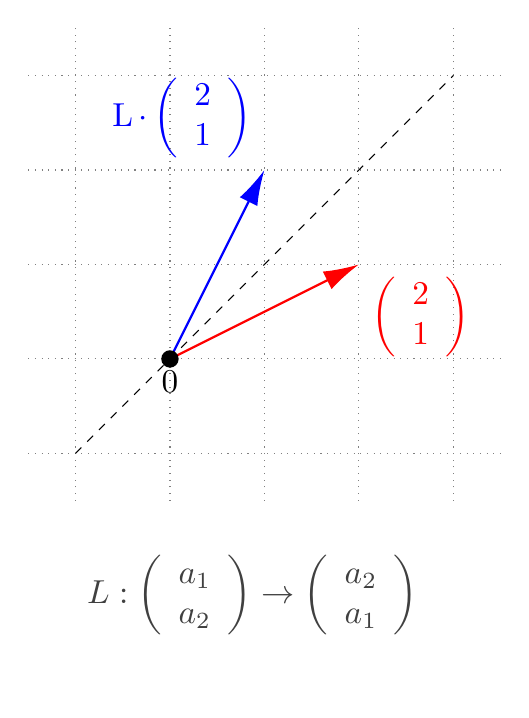
\begin{tikzpicture}[
scale=1.2,
MyPoints/.style={draw=black,fill=black,thick},
Segments/.style={draw=blue!50!red!70,thick},
MyCircles/.style={green!50!blue!50,thin}, 
every node/.style={scale=1.2}
]
\draw[color=gray,step=1.0,dotted] (-1.5,-1.5) grid (3.5,3.5); 
\clip (-1.5,-3.5) rectangle (3.5,3.5);

\pgfmathparse{0}		\let\Xa\pgfmathresult
\pgfmathparse{0}		\let\Ya\pgfmathresult
\coordinate (A) at (\Xa,\Ya);

\pgfmathparse{2}		\let\Xb\pgfmathresult
\pgfmathparse{1}		\let\Yb\pgfmathresult
\coordinate (B) at (\Xb,\Yb);

\pgfmathparse{3}		\let\Xc\pgfmathresult
\pgfmathparse{3}		\let\Yc\pgfmathresult
\coordinate (C) at (\Xc,\Yc);

\pgfmathparse{-1}		\let\Xd\pgfmathresult
\pgfmathparse{-1}		\let\Yd\pgfmathresult
\coordinate (D) at (\Xd,\Yd);

\pgfmathparse{1}		\let\Xe\pgfmathresult
\pgfmathparse{2}		\let\Ye\pgfmathresult
\coordinate (E) at (\Xe,\Ye);



\draw[ black,dashed] (D)--(C);

\draw[-{Latex[length=4.5mm, width=2.5mm]}, >=stealth, veca,thick] (A)--(B) node[below right]{$\left(\begin{array}{l}2 \\ 1\end{array}\right)$};

\draw[-{Latex[length=4.5mm, width=2.5mm]}, >=stealth, vecb,thick] (A)--(E) node[above left]{$\operatorname{L} \cdot \left(\begin{array}{l}2 \\ 1\end{array}\right)$ };

\node [right,darkgray] at (-1,-2.5) {$L:\left(\begin{array}{l}a_{1} \\ a_{2}\end{array}\right) \rightarrow\left(\begin{array}{l}a_{2} \\ a_{1}\end{array}\right)$ }; 


\fill[MyPoints]  (0,0) circle (0.8mm) node [below] {$0$};


\end{tikzpicture}


\subsection{R1.14}

\begin{figure}[H]
	\begin{minipage}[H]{0.5\linewidth}
		
		
		
		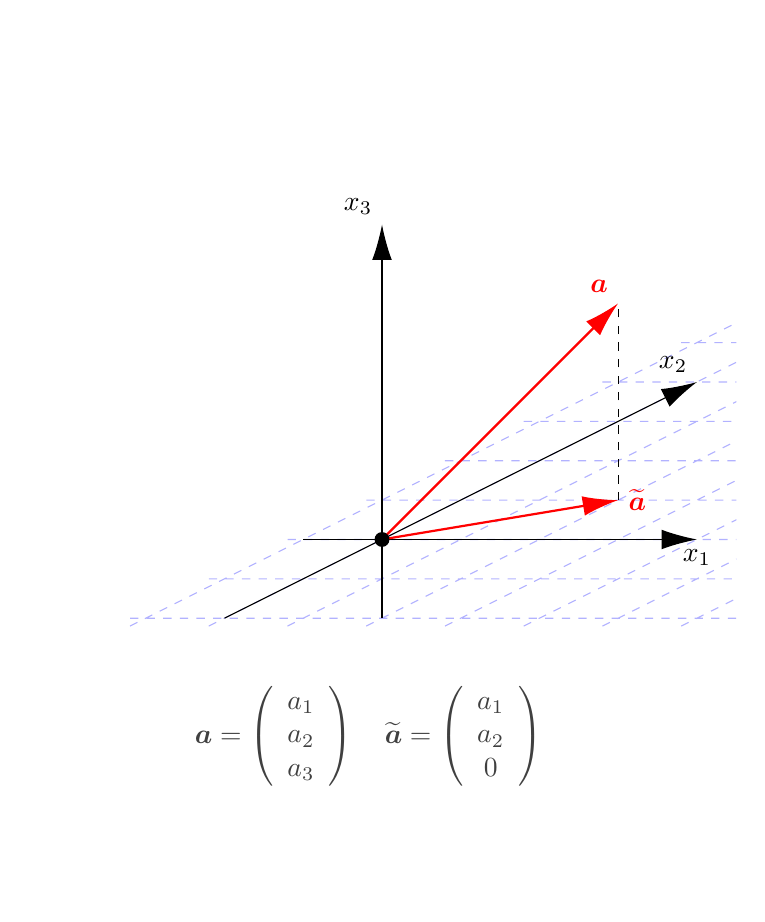
\begin{tikzpicture}[
		scale=1,
		MyPoints/.style={draw=black,fill=black,thick},
		Segments/.style={draw=blue!50!red!70,thick},
		MyCircles/.style={green!50!blue!50,thin}, 
		every node/.style={scale=1}
		]

		\clip (-4.5,-4.5) rectangle (4.5,6.5);

		\begin{scope}[cm={1,0.5,1,0,(0,0)}]
		\draw[draw=blue!30, dashed] (-2.2,-1.2) grid[step=1] (6,7);
		\end{scope}
			
		\draw[-{Latex[length=4.5mm, width=2.5mm]}, >=stealth] (0,-1)--(0,4) node[above left]{$x_3$};
	
		
		\draw[-{Latex[length=4.5mm, width=2.5mm]}, >=stealth] (-1,0)--(4,0) 
		node[below ]{$x_1$};
		
		\draw[-{Latex[length=4.5mm, width=2.5mm]}, >=stealth] (-2,-1)--(4,2) node[above left]{$x_2$};
		
		
		%{\verb!->!new, arrowhead = 2mm, line width=4pt}
		%, arrowhead = 3mm
		%, arrowhead = 0.2
		
		% Feel free to change here coordinates of points A and B
		\pgfmathparse{0}		\let\Xa\pgfmathresult
		\pgfmathparse{0}		\let\Ya\pgfmathresult
		\coordinate (A) at (\Xa,\Ya);
		
		\pgfmathparse{3}		\let\Xb\pgfmathresult
		\pgfmathparse{0.5}		\let\Yb\pgfmathresult
		\coordinate (B) at (\Xb,\Yb);

		\pgfmathparse{3}		\let\Xd\pgfmathresult
		\pgfmathparse{3}		\let\Yd\pgfmathresult
		\coordinate (D) at (\Xd,\Yd);

		
		\pgfmathparse{4}		\let\Xc\pgfmathresult
		\pgfmathparse{0}		\let\Yc\pgfmathresult
		\coordinate (C) at (\Xc,\Yc);
		
		
		\draw[-{Latex[length=4.5mm, width=2.5mm]}, >=stealth, veca, thick] (A)--(B) node[right]{$\widetilde{\ba}$};

		\draw[-{Latex[length=4.5mm, width=2.5mm]}, >=stealth, veca, thick] (A)--(D) node[above left]{$\ba$};

		
		\draw[black, dashed] (B)--(D);
				
		\fill[MyPoints]  (0,0) circle (0.8mm);
		
		\node [right,darkgray] at (-2.5,-2.5) {$\ba=\left(\begin{array}{c}a_{1} \\ a_{2} \\ a_{3}\end{array}\right) \quad \widetilde{\ba}=\left(\begin{array}{c}a_{1} \\ a_{2} \\ 0\end{array}\right)$}; 
		
		
		\end{tikzpicture}
		
		
	\end{minipage}
	\begin{minipage}[H]{0.5\linewidth}
		
		
		\begin{tikzpicture}[
		scale=1,
		MyPoints/.style={draw=blue,fill=blue,thick},
		Segments/.style={draw=blue!50!red!70,thick},
		MyCircles/.style={green!50!blue!50,thin}, 
		every node/.style={scale=1}
		]
		\clip (-4.5,-4.5) rectangle (4.5,6.5);
		
		\draw[color=blue!30,step=1.0,dashed] (-1.5,-1.5) grid (4.5,4.5);
		
		%\draw[->, >=stealth] (-1,0)--(6.5,0) node[right]{$x_1$};
		
		
		\draw[-{Latex[length=4.5mm, width=2.5mm]}, >=stealth] (0,-1)--(0,4) node[above left]{$x_2$};
		
		\draw[-{Latex[length=4.5mm, width=2.5mm]}, >=stealth] (-1,0)--(4,0) 
		node[below]{$x_1$};
		
		
		%{\verb!->!new, arrowhead = 2mm, line width=4pt}
		%, arrowhead = 3mm
		%, arrowhead = 0.2
		
			\pgfmathparse{0}		\let\Xa\pgfmathresult
		\pgfmathparse{0}		\let\Ya\pgfmathresult
		\coordinate (A) at (\Xa,\Ya);
		
		\pgfmathparse{2}		\let\Xb\pgfmathresult
		\pgfmathparse{1}		\let\Yb\pgfmathresult
		\coordinate (B) at (\Xb,\Yb);
		
		\pgfmathparse{3}		\let\Xd\pgfmathresult
		\pgfmathparse{3}		\let\Yd\pgfmathresult
		\coordinate (D) at (\Xd,\Yd);
		
		
		\pgfmathparse{4}		\let\Xc\pgfmathresult
		\pgfmathparse{0}		\let\Yc\pgfmathresult
		\coordinate (C) at (\Xc,\Yc);
		
		
		\draw[-{Latex[length=4.5mm, width=2.5mm]}, >=stealth, veca, thick] (A)--(B) node[above right]{$\operatorname{L} \cdot \ba$};
		
		
		%\draw[black] (A)--(C) node[midway,below]{$4$};
		
	
		\node [right,darkgray] at (0,-2.5) {$\operatorname{L} \ba =\left(\begin{array}{l}a_{1} \\ a_{2} \end{array}\right) $}; 
		
		
		
		\end{tikzpicture}
		
	\end{minipage}
	\hfill
	
\end{figure}



\subsection{R1.15}

\begin{figure}[H]
	
		\begin{minipage}[H]{0.5\linewidth}
		
		
		\begin{tikzpicture}[
		scale=1,
		MyPoints/.style={draw=blue,fill=blue,thick},
		Segments/.style={draw=blue!50!red!70,thick},
		MyCircles/.style={green!50!blue!50,thin}, 
		every node/.style={scale=1}
		]
		\clip (-1.5,-4.5) rectangle (4.5,6.5);
		
		\draw[color=blue!30,step=1.0,dashed] (-1.5,-1.5) grid (4.5,4.5);
		
		%\draw[->, >=stealth] (-1,0)--(6.5,0) node[right]{$x_1$};
		
		
		\draw[-{Latex[length=4.5mm, width=2.5mm]}, >=stealth] (0,-1)--(0,4) node[above left]{$x_2$};
		
		\draw[-{Latex[length=4.5mm, width=2.5mm]}, >=stealth] (-1,0)--(4,0) 
		node[below]{$x_1$};
		
		
		%{\verb!->!new, arrowhead = 2mm, line width=4pt}
		%, arrowhead = 3mm
		%, arrowhead = 0.2
		
		\pgfmathparse{0}		\let\Xa\pgfmathresult
		\pgfmathparse{0}		\let\Ya\pgfmathresult
		\coordinate (A) at (\Xa,\Ya);
		
		\pgfmathparse{2}		\let\Xb\pgfmathresult
		\pgfmathparse{1}		\let\Yb\pgfmathresult
		\coordinate (B) at (\Xb,\Yb);
		
		\pgfmathparse{3}		\let\Xd\pgfmathresult
		\pgfmathparse{3}		\let\Yd\pgfmathresult
		\coordinate (D) at (\Xd,\Yd);
		
		
		\pgfmathparse{4}		\let\Xc\pgfmathresult
		\pgfmathparse{0}		\let\Yc\pgfmathresult
		\coordinate (C) at (\Xc,\Yc);
		
		
		\draw[-{Latex[length=4.5mm, width=2.5mm]}, >=stealth, veca, thick] (A)--(B) node[above right]{$ \ba$};
		
		
		%\draw[black] (A)--(C) node[midway,below]{$4$};
		
		
		\node [right,darkgray] at (0,-2.5) {$ \ba =\left(\begin{array}{l}a_{1} \\ a_{2} \end{array}\right) $}; 
		
		
		
		\end{tikzpicture}
	\end{minipage}
	\begin{minipage}[H]{0.5\linewidth}
		
		
		
		
		\begin{tikzpicture}[
		scale=1,
		MyPoints/.style={draw=black,fill=black,thick},
		Segments/.style={draw=blue!50!red!70,thick},
		MyCircles/.style={green!50!blue!50,thin}, 
		every node/.style={scale=1}
		]
		
		\clip (-3.5,-4.5) rectangle (4.5,6.5);
		
		\begin{scope}[cm={1,0.5,1,0,(0,0)}]
		\draw[draw=blue!30, dashed] (-2.2,-1.2) grid[step=1] (6,7);
		\end{scope}
		
		\draw[-{Latex[length=4.5mm, width=2.5mm]}, >=stealth] (0,-1)--(0,4) node[above left]{$x_3$};
		
		
		\draw[-{Latex[length=4.5mm, width=2.5mm]}, >=stealth] (-1,0)--(4,0) 
		node[below ]{$x_1$};
		
		\draw[-{Latex[length=4.5mm, width=2.5mm]}, >=stealth] (-2,-1)--(4,2) node[above left]{$x_2$};
		
		
		%{\verb!->!new, arrowhead = 2mm, line width=4pt}
		%, arrowhead = 3mm
		%, arrowhead = 0.2
		
		% Feel free to change here coordinates of points A and B
		\pgfmathparse{0}		\let\Xa\pgfmathresult
		\pgfmathparse{0}		\let\Ya\pgfmathresult
		\coordinate (A) at (\Xa,\Ya);
		
		\pgfmathparse{3}		\let\Xb\pgfmathresult
		\pgfmathparse{0.5}		\let\Yb\pgfmathresult
		\coordinate (B) at (\Xb,\Yb);
		
		\pgfmathparse{3}		\let\Xd\pgfmathresult
		\pgfmathparse{3}		\let\Yd\pgfmathresult
		\coordinate (D) at (\Xd,\Yd);
		
		
		\pgfmathparse{4}		\let\Xc\pgfmathresult
		\pgfmathparse{0}		\let\Yc\pgfmathresult
		\coordinate (C) at (\Xc,\Yc);
		
		
		\draw[-{Latex[length=4.5mm, width=2.5mm]}, >=stealth, veca, thick] (A)--(B) node[right]{$ \operatorname{L} \ba$};
		
%		\draw[-{Latex[length=4.5mm, width=2.5mm]}, >=stealth, veca, thick] (A)--(D) node[above left]{$\ba$};
			
%		\draw[black, dashed] (B)--(D);
		
		\fill[MyPoints]  (0,0) circle (0.8mm);
		
		\node [right,darkgray] at (0,-2.5) {$\operatorname{L}  \widetilde{\ba}=\left(\begin{array}{c}a_{1} \\ a_{2} \\ 0\end{array}\right)$}; 
		
		
		\end{tikzpicture}
		
	\end{minipage}
	\hfill
	
\end{figure}



\subsection{R1.16}



\begin{tikzpicture}[
scale=1.2,
MyPoints/.style={draw=blue,fill=blue,thick},
MyPoints2/.style={draw=red,fill=red,thick},
Segments/.style={draw=blue!50!red!70,thick},
MyCircles/.style={green!50!blue!50,thin}, 
every node/.style={scale=1.2}
]
%\grid;
\clip (-1.5,-2.5) rectangle (6.5,5.5);


%%\draw[->, >=stealth] (-1,0)--(6.5,0) node[right]{$x_1$};
%\draw[-{Latex[length=4.5mm, width=2.5mm]}, >=stealth] (0,-1)--(0,5) node[above left]{$x_2$};
%
%\draw[-{Latex[length=4.5mm, width=2.5mm]}, >=stealth] (-1,0)--(6.5,0) 
%node[right]{$x_1$};

% Feel free to change here coordinates of points A and B
\pgfmathparse{0}		\let\Xa\pgfmathresult
\pgfmathparse{0}		\let\Ya\pgfmathresult
\coordinate (A) at (\Xa,\Ya);

\pgfmathparse{2}		\let\Xb\pgfmathresult
\pgfmathparse{3}		\let\Yb\pgfmathresult
\coordinate (B) at (\Xb,\Yb);

\pgfmathparse{3}		\let\Xc\pgfmathresult
\pgfmathparse{1}		\let\Yc\pgfmathresult
\coordinate (C) at (\Xc,\Yc);

\pgfmathparse{5}		\let\Xd\pgfmathresult
\pgfmathparse{4}		\let\Yd\pgfmathresult
\coordinate (D) at (\Xd,\Yd);

\pgfmathparse{2}		\let\Xe\pgfmathresult
\pgfmathparse{0}		\let\Ye\pgfmathresult
\coordinate (E) at (\Xe,\Ye);

\pgfmathparse{5}		\let\Xf\pgfmathresult
\pgfmathparse{0}		\let\Yf\pgfmathresult
\coordinate (F) at (\Xf,\Yf);

\pgfmathparse{5}		\let\Xg\pgfmathresult
\pgfmathparse{-1.5}		\let\Yg\pgfmathresult
\coordinate (G) at (\Xg,\Yg);

\pgfmathparse{0}		\let\Xh\pgfmathresult
\pgfmathparse{-1.5}		\let\Yh\pgfmathresult
\coordinate (H) at (\Xh,\Yh);

\pgfmathparse{-1.5}		\let\Xj\pgfmathresult
\pgfmathparse{0}		\let\Yj\pgfmathresult
\coordinate (J) at (\Xj,\Yj);

\pgfmathparse{6.5}		\let\Xk\pgfmathresult
\pgfmathparse{0}		\let\Yk\pgfmathresult
\coordinate (K) at (\Xk,\Yk);

\pgfmathparse{0}		\let\Xl\pgfmathresult
\pgfmathparse{-1}		\let\Yl\pgfmathresult
\coordinate (L) at (\Xl,\Yl);

\pgfmathparse{5}		\let\Xm\pgfmathresult
\pgfmathparse{-1}		\let\Ym\pgfmathresult
\coordinate (M) at (\Xm,\Ym);



% Let I be the midpoint of [AB]
\pgfmathparse{(\Xb+\Xa)/2} \let\XI\pgfmathresult
\pgfmathparse{(\Yb+\Ya)/2} \let\YI\pgfmathresult
\coordinate (I) at (\XI,\YI);	


\draw[-{Latex[length=4.5mm, width=2.5mm]}, >=stealth, veca,thick] (A)--(B) node[midway,left]{$\ba$};

\draw[-{Latex[length=4.5mm, width=1.5mm]}, >=stealth, veca,thick] (B)--(D) node[midway,above]{$\bb$};

\draw[-{Latex[length=4.5mm, width=2.5mm]}, >=stealth, vecc,thick] (A)--(D) node[below right]{$\ba+\bb$};

\draw[dashed] (B)--(E);
\draw[dashed] (D)--(F);
\draw[dashed] (J)--(K);

\draw[-{Latex[length=4.5mm, width=1.5mm]}, >=stealth, vecb,thick] (A)--(E) node[midway,below]{$\operatorname{H} \ba$};

\draw[-{Latex[length=4.5mm, width=1.5mm]}, >=stealth, vecb,thick] (E)--(F) node[midway,below]{$\operatorname{H} \bb$};

\draw[-{Latex[length=4.5mm, width=1.5mm]}, >=stealth, vecb,thick] (L)--(M) node[midway,below]{$\operatorname{H} (\ba+\bb)$};



\draw[thick] (F)--(G);
\draw[thick] (A)--(H);


\fill[MyPoints]  (L) circle (0.8mm);
\fill[MyPoints2]  (A) circle (0.8mm);


\end{tikzpicture}


\subsection{R1.17}



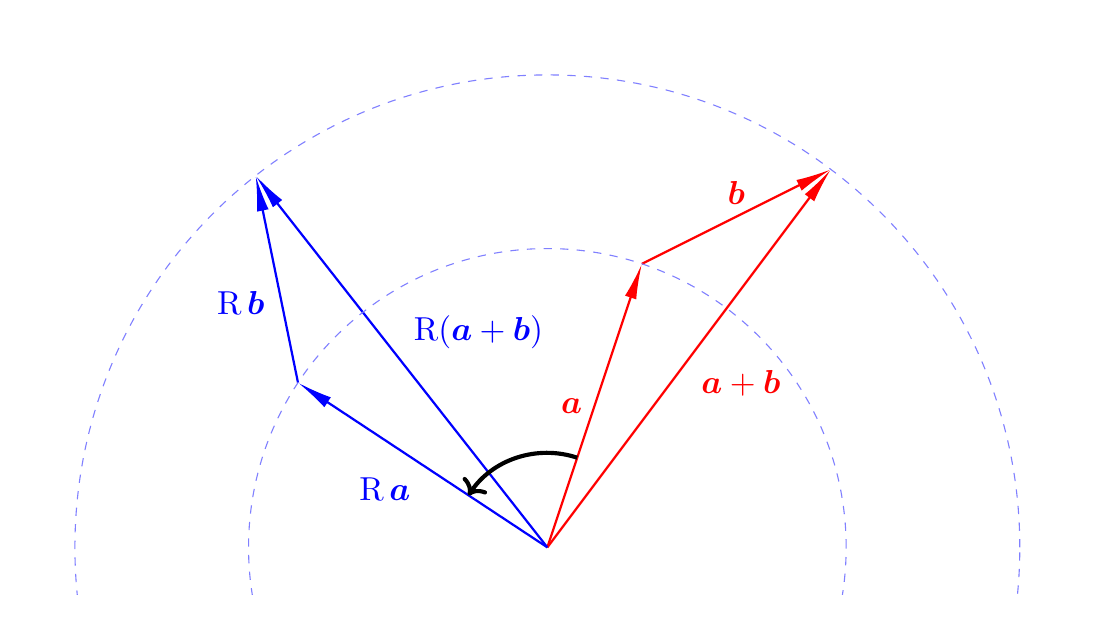
\begin{tikzpicture}[
scale=1.2,
MyPoints/.style={draw=blue,fill=white,thick},
Segments/.style={draw=blue!50!red!70,thick},
MyCircles/.style={blue!50,dashed}, 
every node/.style={scale=1.2}
]
%\grid;
%\draw[color=gray,step=1.0,dotted] (-7.1,-2.1) grid (7.6,6.1);
\clip (-5.5,-.5) rectangle (5.5,5.5);


%%\draw[->, >=stealth] (-1,0)--(6.5,0) node[right]{$x_1$};
%\draw[-{Latex[length=4.5mm, width=2.5mm]}, >=stealth] (0,-1)--(0,5) node[above left]{$x_2$};
%
%\draw[-{Latex[length=4.5mm, width=2.5mm]}, >=stealth] (-1,0)--(6.5,0) 
%node[right]{$x_1$};

% Feel free to change here coordinates of points A and B
\pgfmathparse{0}		\let\Xa\pgfmathresult
\pgfmathparse{0}		\let\Ya\pgfmathresult
\coordinate (A) at (\Xa,\Ya);

\pgfmathparse{1}		\let\Xb\pgfmathresult
\pgfmathparse{3}		\let\Yb\pgfmathresult
\coordinate (B) at (\Xb,\Yb);

\pgfmathparse{3}		\let\Xc\pgfmathresult
\pgfmathparse{1}		\let\Yc\pgfmathresult
\coordinate (C) at (\Xc,\Yc);

\pgfmathparse{3}		\let\Xd\pgfmathresult
\pgfmathparse{4}		\let\Yd\pgfmathresult
\coordinate (D) at (\Xd,\Yd);

\pgfmathparse{75}		\let\angle\pgfmathresult;
\pgfmathparse{sqrt(10)}		\let\rad\pgfmathresult;


\pgfmathparse{\Xb*cos(\angle)  - \Yb*sin(\angle)}		\let\Xe\pgfmathresult
\pgfmathparse{\Xb*sin(\angle)  + \Yb*cos(\angle)}		\let\Ye\pgfmathresult
\coordinate (E) at (\Xe,\Ye);

\pgfmathparse{\Xd*cos(\angle)  - \Yd*sin(\angle)}		\let\Xf\pgfmathresult
\pgfmathparse{\Xd*sin(\angle)  + \Yd*cos(\angle)}		\let\Yf\pgfmathresult
\coordinate (F) at (\Xf,\Yf);


% Let I be the midpoint of [AB]
\pgfmathparse{(\Xb+\Xa)/2} \let\XI\pgfmathresult
\pgfmathparse{(\Yb+\Ya)/2} \let\YI\pgfmathresult
\coordinate (I) at (\XI,\YI);	


\draw[-{Latex[length=4.5mm, width=1.5mm]}, >=stealth, veca,thick] (A)--(B) node[midway,left]{$\ba$};

\draw[-{Latex[length=4.5mm, width=1.5mm]}, >=stealth, veca,thick] (B)--(D) node[midway,above]{$\bb$};

\draw[-{Latex[length=4.5mm, width=1.5mm]}, >=stealth, veca,thick] (A)--(D) node[midway,below right]{$\ba+\bb$};

\draw[-{Latex[length=4.5mm, width=1.5mm]}, >=stealth, vecb,thick] (A)--(E) node[midway,below left]{$\operatorname{R} \ba$};

\draw[-{Latex[length=4.5mm, width=1.5mm]}, >=stealth, vecb,thick] (E)--(F) node[midway,below left]{$\operatorname{R} \bb$};

\draw[-{Latex[length=4.5mm, width=1.5mm]}, >=stealth, vecb,thick] (A)--(F) node[midway,above right]{$\operatorname{R} (\ba+\bb)$};

\draw[MyCircles] (A) circle ({\rad});

\draw[MyCircles] (A) circle ({5});

\tkzMarkAngle[size=1, mark = none, arrows=->,line width=1.5pt, mkcolor=red ](B,A,E);


\end{tikzpicture}




\subsection{R1.18}



\begin{tikzpicture}[
scale=1.2,
MyPoints/.style={draw=blue,fill=white,thick},
Segments/.style={draw=blue!50!red!70,thick},
MyCircles/.style={green!50!blue!50,thin}, 
every node/.style={scale=1.2}
]
%\grid;
\clip (-1.5,-1.5) rectangle (5.5,5.5);

\pgfmathparse{2}		\let\Xa\pgfmathresult
\pgfmathparse{2}		\let\Ya\pgfmathresult
\coordinate (A) at (\Xa,\Ya);

\pgfmathparse{5}		\let\Xb\pgfmathresult
\pgfmathparse{5}		\let\Yb\pgfmathresult
\coordinate (B) at (\Xb,\Yb);

\pgfmathparse{-1}		\let\Xc\pgfmathresult
\pgfmathparse{5}		\let\Yc\pgfmathresult
\coordinate (C) at (\Xc,\Yc);

\pgfmathparse{4}		\let\Xd\pgfmathresult
\pgfmathparse{0}		\let\Yd\pgfmathresult
\coordinate (D) at (\Xd,\Yd);

\pgfmathparse{0}		\let\Xe\pgfmathresult
\pgfmathparse{4}		\let\Ye\pgfmathresult
\coordinate (E) at (\Xe,\Ye);

\pgfmathparse{3.5}		\let\Xf\pgfmathresult
\pgfmathparse{3.5}		\let\Yf\pgfmathresult
\coordinate (F) at (\Xf,\Yf);

\pgfmathparse{4}		\let\Xg\pgfmathresult
\pgfmathparse{4}		\let\Yg\pgfmathresult
\coordinate (G) at (\Xg,\Yg);

\pgfmathparse{4.5}		\let\Xh\pgfmathresult
\pgfmathparse{4.5}		\let\Yh\pgfmathresult
\coordinate (H) at (\Xh,\Yh);


\draw[ black,dashed] (D)--(C);

\draw[dashed] (A)--(B);

\draw[-{Latex[length=4.5mm, width=2.5mm]}, >=stealth, vecb,thick] (E)--(A) node[midway,below left]{$\bb$};

\draw[-{Latex[length=4.5mm, width=2.5mm]}, >=stealth, veca,thick] (E)--(F) node[right]{$\bv ?$};

\draw[-{Latex[length=4.5mm, width=2.5mm]}, >=stealth, veca,thick] (E)--(G) node[right]{$\bv ?$};

\draw[-{Latex[length=4.5mm, width=2.5mm]}, >=stealth, veca,thick] (E)--(H) node[right]{$\bv ?$};

\node [above right] at (0, 5) {$\operatorname{H} \bv = \bb$}; 


\end{tikzpicture}



\subsection{R1.19}



\begin{tikzpicture}[
scale=1.2,
MyPoints/.style={draw=blue,fill=white,thick},
Segments/.style={draw=blue!50!red!70,thick},
MyCircles/.style={blue!50,dashed}, 
every node/.style={scale=1.2}
]
%\grid;
%\draw[color=gray,step=1.0,dotted] (-7.1,-2.1) grid (7.6,6.1);
\clip (-5.5,-.5) rectangle (5.5,5.5);


%%\draw[->, >=stealth] (-1,0)--(6.5,0) node[right]{$x_1$};
%\draw[-{Latex[length=4.5mm, width=2.5mm]}, >=stealth] (0,-1)--(0,5) node[above left]{$x_2$};
%
%\draw[-{Latex[length=4.5mm, width=2.5mm]}, >=stealth] (-1,0)--(6.5,0) 
%node[right]{$x_1$};

% Feel free to change here coordinates of points A and B
\pgfmathparse{0}		\let\Xa\pgfmathresult
\pgfmathparse{0}		\let\Ya\pgfmathresult
\coordinate (A) at (\Xa,\Ya);

\pgfmathparse{1.5}		\let\Xb\pgfmathresult
\pgfmathparse{3}		\let\Yb\pgfmathresult
\coordinate (B) at (\Xb,\Yb);

\pgfmathparse{3}		\let\Xc\pgfmathresult
\pgfmathparse{1}		\let\Yc\pgfmathresult
\coordinate (C) at (\Xc,\Yc);

\pgfmathparse{3}		\let\Xd\pgfmathresult
\pgfmathparse{4}		\let\Yd\pgfmathresult
\coordinate (D) at (\Xd,\Yd);

\pgfmathparse{75}		\let\angle\pgfmathresult;
\pgfmathparse{sqrt(10)}		\let\rad\pgfmathresult;


\pgfmathparse{\Xb*cos(\angle)  - \Yb*sin(\angle)}		\let\Xe\pgfmathresult
\pgfmathparse{\Xb*sin(\angle)  + \Yb*cos(\angle)}		\let\Ye\pgfmathresult
\coordinate (E) at (\Xe,\Ye);

\pgfmathparse{\Xd*cos(\angle)  - \Yd*sin(\angle)}		\let\Xf\pgfmathresult
\pgfmathparse{\Xd*sin(\angle)  + \Yd*cos(\angle)}		\let\Yf\pgfmathresult
\coordinate (F) at (\Xf,\Yf);


% Let I be the midpoint of [AB]
\pgfmathparse{(\Xb+\Xa)/2} \let\XI\pgfmathresult
\pgfmathparse{(\Yb+\Ya)/2} \let\YI\pgfmathresult
\coordinate (I) at (\XI,\YI);	


\draw[-{Latex[length=4.5mm, width=1.5mm]}, >=stealth, veca,thick] (A)--(B) node[midway,right]{$\bv$};


\draw[-{Latex[length=4.5mm, width=1.5mm]}, >=stealth, vecb,thick] (A)--(E) node[midway,below left]{$\bb$};

\tkzMarkAngle[size=1, mark = none, arrows=->,line width=1.5pt, mkcolor=red ](B,A,E);

\draw[dashed] (B) to[bend right] (E);

\node [above right] at (-0.5, 1) {$\operatorname{R}$}; 

\node [above right] at (-2, 4) {$\operatorname{R} \bv = \bb$}; 


\end{tikzpicture}






\subsection{R1.20}


\begin{tikzpicture}[
scale=1.2,
MyPoints/.style={draw=blue,fill=white,thick},
Segments/.style={draw=blue!50!red!70,thick},
MyCircles/.style={green!50!blue!50,thin}, 
every node/.style={scale=1.2}
]
%\grid;
\clip (-.5,-.5) rectangle (6.5,5.5);


%%\draw[->, >=stealth] (-1,0)--(6.5,0) node[right]{$x_1$};
%\draw[-{Latex[length=4.5mm, width=2.5mm]}, >=stealth] (0,-1)--(0,5) node[above left]{$x_2$};
%
%\draw[-{Latex[length=4.5mm, width=2.5mm]}, >=stealth] (-1,0)--(6.5,0) 
%node[right]{$x_1$};

% Feel free to change here coordinates of points A and B
\pgfmathparse{0}		\let\Xa\pgfmathresult
\pgfmathparse{0}		\let\Ya\pgfmathresult
\coordinate (A) at (\Xa,\Ya);

\pgfmathparse{5}		\let\Xb\pgfmathresult
\pgfmathparse{0}		\let\Yb\pgfmathresult
\coordinate (B) at (\Xb,\Yb);

\pgfmathparse{2.5}		\let\Xc\pgfmathresult
\pgfmathparse{5}		\let\Yc\pgfmathresult
\coordinate (C) at (\Xc,\Yc);

\pgfmathparse{1.5}		\let\Xd\pgfmathresult
\pgfmathparse{3}		\let\Yd\pgfmathresult
\coordinate (D) at (\Xd,\Yd);

\pgfmathparse{2}		\let\Xe\pgfmathresult
\pgfmathparse{1.5}		\let\Ye\pgfmathresult
\coordinate (E) at (\Xe,\Ye);



% Let I be the midpoint of [AB]
\pgfmathparse{(\Xb+\Xa)/2} \let\XI\pgfmathresult
\pgfmathparse{(\Yb+\Ya)/2} \let\YI\pgfmathresult
\coordinate (I) at (\XI,\YI);	


\draw[-{Latex[length=4.5mm, width=2.5mm]}, >=stealth, darkgray,thick] (A)--(B) node[above]{$\operatorname{L} \bb \neq \lambda \bb$};


\draw[-{Latex[length=4.5mm, width=2.5mm]}, >=stealth, vecb,thick] (A)--(E) node[midway,below]{$\bb$};


\draw[-{Latex[length=4.5mm, width=2.5mm]}, >=stealth, darkgray,thick] (A)--(C) node[above]{$\operatorname{L} \ba = \lambda \ba$};

\draw[-{Latex[length=4.5mm, width=2.5mm]}, >=stealth, veca,thick] (A)--(D) node[midway,left]{$\ba$};








\end{tikzpicture}


\section{Лекция 2}

\subsection{R2.1}


\begin{tikzpicture}[
scale=1.2,
MyPoints/.style={draw=blue,fill=white,thick},
Segments/.style={draw=blue!50!red!70,thick},
MyCircles/.style={green!50!blue!50,thin}, 
every node/.style={scale=1.2}
]
%\grid;
\clip (-.5,-.5) rectangle (7.5,6.5);


%%\draw[->, >=stealth] (-1,0)--(6.5,0) node[right]{$x_1$};
%\draw[-{Latex[length=4.5mm, width=2.5mm]}, >=stealth] (0,-1)--(0,5) node[above left]{$x_2$};
%
%\draw[-{Latex[length=4.5mm, width=2.5mm]}, >=stealth] (-1,0)--(6.5,0) 
%node[right]{$x_1$};

% Feel free to change here coordinates of points A and B
\pgfmathparse{0}		\let\Xa\pgfmathresult
\pgfmathparse{0}		\let\Ya\pgfmathresult
\coordinate (A) at (\Xa,\Ya);

\pgfmathparse{1}		\let\Xb\pgfmathresult
\pgfmathparse{3}		\let\Yb\pgfmathresult
\coordinate (B) at (\Xb,\Yb);

\pgfmathparse{3}		\let\Xc\pgfmathresult
\pgfmathparse{1}		\let\Yc\pgfmathresult
\coordinate (C) at (\Xc,\Yc);

\pgfmathparse{7}		\let\Xd\pgfmathresult
\pgfmathparse{5}		\let\Yd\pgfmathresult
\coordinate (D) at (\Xd,\Yd);

\pgfmathparse{6}		\let\Xe\pgfmathresult
\pgfmathparse{2}		\let\Ye\pgfmathresult
\coordinate (E) at (\Xe,\Ye);


% Let I be the midpoint of [AB]
\pgfmathparse{(\Xb+\Xa)/2} \let\XI\pgfmathresult
\pgfmathparse{(\Yb+\Ya)/2} \let\YI\pgfmathresult
\coordinate (I) at (\XI,\YI);	


\draw[-{Latex[length=4.5mm, width=2mm]}, >=stealth, vecb,thick] (A)--(B) node[midway,left]{$\bb$};

\draw[vecb,dashed] (E)--(D);


\draw[-{Latex[length=4.5mm, width=2mm]}, >=stealth, veca,thick] (A)--(C) node[midway,below]{$\ba$};

\draw[ veca,dashed] (C)--(E) node[midway,below]{$\ba$};


\draw[veca,dashed] (B)--(D);


\draw[-{Latex[length=4.5mm, width=2.5mm]}, >=stealth, vecc,thick] (A)--(D) node[midway,above]{$\bc$};


\node [above right] at (2, 5) {$\bc = 2 \cdot \ba + 1 \cdot \bb $}; 


\end{tikzpicture}



\subsection{R2.2}



\begin{tikzpicture}[
scale=1,
MyPoints/.style={draw=black,fill=black,thick},
Segments/.style={draw=blue!50!red!70,thick},
MyCircles/.style={green!50!blue!50,thin}, 
every node/.style={scale=1}
]

%\grid;

\clip (-1.5,-4.5) rectangle (5.5,5.5);

\begin{scope}[cm={1,1,1.5,0,(0,0)}]
\draw[draw=blue!30, dashed] (-1.2,-4.2) grid[step=1] (3.5,7);
\end{scope}

%{\verb!->!new, arrowhead = 2mm, line width=4pt}
%, arrowhead = 3mm
%, arrowhead = 0.2

% Feel free to change here coordinates of points A and B
\pgfmathparse{0}		\let\Xa\pgfmathresult
\pgfmathparse{0}		\let\Ya\pgfmathresult
\coordinate (A) at (\Xa,\Ya);

\pgfmathparse{2}		\let\Xb\pgfmathresult
\pgfmathparse{0.5}		\let\Yb\pgfmathresult
\coordinate (B) at (\Xb,\Yb);

\pgfmathparse{2}		\let\Xd\pgfmathresult
\pgfmathparse{4}		\let\Yd\pgfmathresult
\coordinate (D) at (\Xd,\Yd);

\pgfmathparse{4}		\let\Xc\pgfmathresult
\pgfmathparse{0}		\let\Yc\pgfmathresult
\coordinate (C) at (\Xc,\Yc);


\pgfmathparse{1}		\let\Xe\pgfmathresult
\pgfmathparse{1}		\let\Ye\pgfmathresult
\coordinate (E) at (\Xe,\Ye);

\pgfmathparse{2.5}		\let\Xf\pgfmathresult
\pgfmathparse{0}		\let\Yf\pgfmathresult
\coordinate (F) at (\Xf,\Yf);

\pgfmathparse{4}		\let\Xg\pgfmathresult
\pgfmathparse{1}		\let\Yg\pgfmathresult
\coordinate (G) at (\Xg,\Yg);




\draw[-{Latex[length=4.5mm, width=2.5mm]}, >=stealth, thick] (A)--(D) node[above left]{$\bd$};

\draw[-{Latex[length=4.5mm, width=2.5mm]}, >=stealth, vecb, thick] (A)--(E) node[right]{$\ba$};

\draw[-{Latex[length=4.5mm, width=2.5mm]}, >=stealth, vecb, thick] (A)--(F) node[below]{$\bb$};

\draw[-{Latex[length=4.5mm, width=2.5mm]}, >=stealth, veca, thick] (A)--(G) node[right]{$\bc$};


\draw[black, dashed] (B)--(D);

\fill[MyPoints]  (0,0) circle (0.8mm);

\node [right,darkgray] at (-0.5,-2) {$\{\ba, \bb, \bc\}$ -- линейно зависимы}; 

\node [right,darkgray] at (-0.5,-3) {$\{\ba, \bb, \bd\}$ -- независимы}; 



\end{tikzpicture}




\subsection{R2.3}



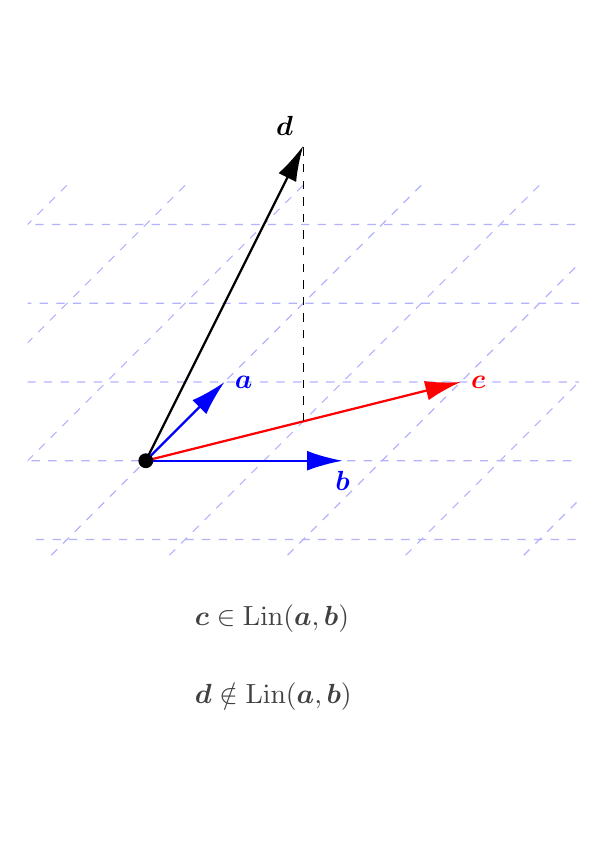
\begin{tikzpicture}[
scale=1,
MyPoints/.style={draw=black,fill=black,thick},
Segments/.style={draw=blue!50!red!70,thick},
MyCircles/.style={green!50!blue!50,thin}, 
every node/.style={scale=1}
]

%\grid;

\clip (-1.5,-4.5) rectangle (5.5,5.5);

\begin{scope}[cm={1,1,1.5,0,(0,0)}]
\draw[draw=blue!30, dashed] (-1.2,-4.2) grid[step=1] (3.5,7);
\end{scope}

%{\verb!->!new, arrowhead = 2mm, line width=4pt}
%, arrowhead = 3mm
%, arrowhead = 0.2

% Feel free to change here coordinates of points A and B
\pgfmathparse{0}		\let\Xa\pgfmathresult
\pgfmathparse{0}		\let\Ya\pgfmathresult
\coordinate (A) at (\Xa,\Ya);

\pgfmathparse{2}		\let\Xb\pgfmathresult
\pgfmathparse{0.5}		\let\Yb\pgfmathresult
\coordinate (B) at (\Xb,\Yb);

\pgfmathparse{2}		\let\Xd\pgfmathresult
\pgfmathparse{4}		\let\Yd\pgfmathresult
\coordinate (D) at (\Xd,\Yd);

\pgfmathparse{4}		\let\Xc\pgfmathresult
\pgfmathparse{0}		\let\Yc\pgfmathresult
\coordinate (C) at (\Xc,\Yc);


\pgfmathparse{1}		\let\Xe\pgfmathresult
\pgfmathparse{1}		\let\Ye\pgfmathresult
\coordinate (E) at (\Xe,\Ye);

\pgfmathparse{2.5}		\let\Xf\pgfmathresult
\pgfmathparse{0}		\let\Yf\pgfmathresult
\coordinate (F) at (\Xf,\Yf);

\pgfmathparse{4}		\let\Xg\pgfmathresult
\pgfmathparse{1}		\let\Yg\pgfmathresult
\coordinate (G) at (\Xg,\Yg);




\draw[-{Latex[length=4.5mm, width=2.5mm]}, >=stealth, thick] (A)--(D) node[above left]{$\bd$};

\draw[-{Latex[length=4.5mm, width=2.5mm]}, >=stealth, vecb, thick] (A)--(E) node[right]{$\ba$};

\draw[-{Latex[length=4.5mm, width=2.5mm]}, >=stealth, vecb, thick] (A)--(F) node[below]{$\bb$};

\draw[-{Latex[length=4.5mm, width=2.5mm]}, >=stealth, veca, thick] (A)--(G) node[right]{$\bc$};


\draw[black, dashed] (B)--(D);

\fill[MyPoints]  (0,0) circle (0.8mm);

\node [right,darkgray] at (0.5,-2) {$\bc \in \operatorname{Lin} (\ba, \bb) $ }; 

\node [right,darkgray] at (0.5,-3) {$\bd \notin \operatorname{Lin} (\ba, \bb) $ }; 



\end{tikzpicture}


\subsection{R2.4}


\begin{tikzpicture}[
scale=1,
MyPoints/.style={draw=blue,fill=white,thick},
Segments/.style={draw=blue!50!red!70,thick},
MyCircles/.style={green!50!blue!50,thin}, 
every node/.style={scale=1}
]
%\grid;
\clip (-5.5,-2.5) rectangle (7.5,5.5);


%\draw[->, >=stealth] (-1,0)--(6.5,0) node[right]{$x_1$};
\draw[-{Latex[length=4.5mm, width=2.5mm]}, >=stealth] (0,-1)--(0,5) node[above left]{$x_2$};

\draw[-{Latex[length=4.5mm, width=2.5mm]}, >=stealth] (-4,0)--(6.5,0) 
node[right]{$x_1$};


%{\verb!->!new, arrowhead = 2mm, line width=4pt}
%, arrowhead = 3mm
%, arrowhead = 0.2

% Feel free to change here coordinates of points A and B
\pgfmathparse{0}		\let\Xa\pgfmathresult
\pgfmathparse{0}		\let\Ya\pgfmathresult
\coordinate (A) at (\Xa,\Ya);

\pgfmathparse{4}		\let\Xb\pgfmathresult
\pgfmathparse{3}		\let\Yb\pgfmathresult
\coordinate (B) at (\Xb,\Yb);

\pgfmathparse{4}		\let\Xc\pgfmathresult
\pgfmathparse{0}		\let\Yc\pgfmathresult
\coordinate (C) at (\Xc,\Yc);




\node [above right,darkgray] at (1,3.5) {$\det \operatorname{L} = \dfrac{\text{площадь*} (\operatorname{LF})}{\text{площадь*} (\operatorname{F})} $};



\pgfmathparse{4}		\let\Xg\pgfmathresult
\pgfmathparse{0}		\let\Yg\pgfmathresult
\coordinate (G) at (\Xg,\Yg);

\pgfmathparse{4}		\let\Xh\pgfmathresult
\pgfmathparse{0}		\let\Yh\pgfmathresult
\coordinate (H) at (\Xh,\Yh);

\pgfmathparse{4}		\let\Xi\pgfmathresult
\pgfmathparse{0}		\let\Yi\pgfmathresult
\coordinate (I) at (\Xi,\Yi);



\begin{scope}[cm={1,1,1.5,0.5,(0,0)}]
\draw[pattern=north west lines, pattern color=blue!50, draw=none ] (0,0) rectangle (2,2);
\draw[-{Latex[length=4.5mm, width=2.5mm]}, >=stealth, vecb,thick] (0,0)--(0,2) node[below]{$\ba$};
\draw[-{Latex[length=4.5mm, width=2.5mm]}, >=stealth, vecb,thick] (0,0)--(2,0) node[above]{$\bb$};
\end{scope};


\pgfmathparse{3}		\let\Xd\pgfmathresult
\pgfmathparse{1}		\let\Yd\pgfmathresult
\coordinate (D) at (\Xd,\Yd);

\pgfmathparse{0}		\let\Xe\pgfmathresult
\pgfmathparse{0}		\let\Ye\pgfmathresult
\coordinate (E) at (\Xe,\Ye);

\pgfmathparse{2}		\let\Xf\pgfmathresult
\pgfmathparse{2}		\let\Yf\pgfmathresult
\coordinate (F) at (\Xf,\Yf);


\tkzMarkAngle[size=1, mark = none, arrows=->,line width=1pt, mkcolor=blue ](D,E,F);


\begin{scope}[cm={-1,2,-1.5,0.5,(0,0)}]
\draw[pattern=north west lines,pattern color=black!50, draw=none ] (0,0) rectangle (0.9,2);
\draw[-{Latex[length=4.5mm, width=2.5mm]}, >=stealth, thick] (0,0)--(0,2) node[below]{$\operatorname{L} \ba$};
\draw[-{Latex[length=4.5mm, width=2.5mm]}, >=stealth, thick] (0,0)--(0.9,0) node[above]{$\operatorname{L} \bb$};

\end{scope}



\pgfmathparse{-1}		\let\Xg\pgfmathresult
\pgfmathparse{2}		\let\Yg\pgfmathresult
\coordinate (G) at (\Xg,\Yg);

\pgfmathparse{-3}		\let\Xi\pgfmathresult
\pgfmathparse{1}		\let\Yi\pgfmathresult
\coordinate (I) at (\Xi,\Yi);

\tkzMarkAngle[size=1, mark = none, arrows=->,line width=1pt, mkcolor=blue ](G,E,I);

\node [right,darkgray] at (-2.5,1.5) {$\operatorname{LF}$ }; 

\node [right,darkgray] at (2,1.5) {$\operatorname{F}$ }; 


%\tkzMarkAngle[size=1, mark = none, arrows=->,line width=1.5pt, mkcolor=red ](B,A,E);



\end{tikzpicture}



\subsection{R2.5}


\begin{tikzpicture}[
scale=1,
MyPoints/.style={draw=blue,fill=white,thick},
Segments/.style={draw=blue!50!red!70,thick},
MyCircles/.style={green!50!blue!50,thin}, 
every node/.style={scale=1.2}
]
%\draw[color=gray,step=1.0,dotted] (-5.5,-6.5) grid (5.5,6.5); 
\clip (-5.5,-6.5) rectangle (8.1,6.5);

%{\verb!->!new, arrowhead = 2mm, line width=4pt}
%, arrowhead = 3mm
%, arrowhead = 0.2

% Feel free to change here coordinates of points A and B
\pgfmathparse{0}		\let\Xa\pgfmathresult
\pgfmathparse{0}		\let\Ya\pgfmathresult
\coordinate (A) at (\Xa,\Ya);

\pgfmathparse{0}		\let\Xb\pgfmathresult
\pgfmathparse{3}		\let\Yb\pgfmathresult
\coordinate (B) at (\Xb,\Yb);

\pgfmathparse{2}		\let\Xc\pgfmathresult
\pgfmathparse{2}		\let\Yc\pgfmathresult
\coordinate (C) at (\Xc,\Yc);

\pgfmathparse{4}		\let\Xd\pgfmathresult
\pgfmathparse{0}		\let\Yd\pgfmathresult
\coordinate (D) at (\Xd,\Yd);

\pgfmathparse{2}		\let\Xe\pgfmathresult
\pgfmathparse{5}		\let\Ye\pgfmathresult
\coordinate (E) at (\Xe,\Ye);

\pgfmathparse{6}		\let\Xf\pgfmathresult
\pgfmathparse{5}		\let\Yf\pgfmathresult
\coordinate (F) at (\Xf,\Yf);

\pgfmathparse{4}		\let\Xg\pgfmathresult
\pgfmathparse{3}		\let\Yg\pgfmathresult
\coordinate (G) at (\Xg,\Yg);

\pgfmathparse{6}		\let\Xg\pgfmathresult
\pgfmathparse{2}		\let\Yg\pgfmathresult
\coordinate (H) at (\Xg,\Yg);


\draw[-{Latex[length=4.5mm, width=2.5mm]}, >=stealth, vecb,  thick] (A)--(B) node[midway, left]{$\ba$};

\draw[-{Latex[length=4.5mm, width=2.5mm]}, >=stealth, vecb,  thick] (A)--(C) node[midway, above]{$\bb$};

\draw[-{Latex[length=4.5mm, width=2.5mm]}, >=stealth, vecb,  thick] (A)--(D) node[midway, below]{$\bc$};

\draw[vecb, dashed] (C)--(E);
\draw[vecb, dashed] (B)--(E);
\draw[vecb, dashed] (E)--(F);
\draw[vecb, dashed] (G)--(F);
\draw[vecb, dashed] (G)--(B);
\draw[vecb, dashed] (G)--(D);
\draw[vecb, dashed] (D)--(H);
\draw[vecb, dashed] (F)--(H);
\draw[vecb, dashed] (C)--(H);

\begin{scope}[cm={0.1,-0.9,-1,0,(0,0)}]
\draw[-{Latex[length=4.5mm, width=2.5mm]}, >=stealth,   thick] (0,0)--(0,3) node[midway, above]{$\operatorname{L} \ba$};
\draw[-{Latex[length=4.5mm, width=2.5mm]}, >=stealth,   thick] (0,0)--(2,2) node[midway, above left ]{$\operatorname{L} \bb$};
\draw[-{Latex[length=4.5mm, width=2.5mm]}, >=stealth,   thick] (0,0)--(4,0) node[midway, right]{$\operatorname{L} \bc$};
\draw[vecb, dashed] (2,2)--(2,5);
\draw[vecb, dashed] (0,3)--(2,5);
\draw[vecb, dashed] (2,5)--(6,5);
\draw[vecb, dashed] (4,3)--(6,5);
\draw[vecb, dashed] (4,3)--(0,3);
\draw[vecb, dashed] (4,3)--(4,0);
\draw[vecb, dashed] (4,0)--(6,2);
\draw[vecb, dashed] (6,5)--(6,2);
\draw[vecb, dashed] (2,2)--(6,2);
\end{scope}



\node [right,darkgray] at (-5,-6) {$\operatorname{LF}$ }; 

\node [right,darkgray] at (5,5.5) {$\operatorname{F}$ }; 



%\draw[-{Latex[length=4.5mm, width=2.5mm]}, >=stealth, thick] (A)--(B) node[left]{$\ba$};
%
%\draw[-{Latex[length=4.5mm, width=2.5mm]}, >=stealth, thick] (A)--(C) node[above]{$\bb$};
%
%\draw[-{Latex[length=4.5mm, width=2.5mm]}, >=stealth, thick] (A)--(D) node[above]{$\bc$};

\node [above right,darkgray] at (2,-3.5) {$\det \operatorname{L} = \dfrac{\text{объем*} (\operatorname{LF})}{\text{объем*} (\operatorname{F})} $};





\end{tikzpicture}



\end{document}



